% !TeX program = xelatex
% Reusable Chinese doctoral-thesis template for PDF and DOCX conversion.
\documentclass[UTF8,zihao=-4,openany,twoside]{ctexbook}

\usepackage[a4paper,top=2.54cm,bottom=2.54cm,left=3.17cm,right=3.17cm,
  headheight=15pt,headsep=0.80cm,footskip=1.10cm]{geometry}
\usepackage{fontspec}
\usepackage{amsmath,amssymb,bm}
\usepackage{newtxmath} % Times-compatible math; full symbol and delimiter support.
\usepackage{graphicx}
\usepackage{eso-pic}
\usepackage{expl3}
\usepackage{booktabs,longtable,array}
\setlength{\heavyrulewidth}{1.5bp}
\setlength{\lightrulewidth}{0.5bp}
\usepackage{tabularx}
\newcolumntype{Y}{>{\centering\arraybackslash}X}
\usepackage{caption}
\usepackage{fancyhdr}
\usepackage{emptypage}
\usepackage{setspace}
\setlength{\intextsep}{18bp plus 2bp minus 2bp}
\setlength{\textfloatsep}{12bp plus 2bp minus 2bp}
\setlength{\floatsep}{18bp plus 2bp minus 2bp}
% Figures: 18 bp before, 12 bp after. Tables: 12 bp on both sides.
\AddToHook{env/figure/before}{\setlength{\intextsep}{18bp plus 2bp minus 2bp}}
\AddToHook{env/figure/end}{\global\intextsep=12bp plus 2bp minus 2bp\relax}
\AddToHook{env/table/before}{\setlength{\intextsep}{12bp plus 2bp minus 2bp}}
\usepackage[hidelinks,bookmarksnumbered=true]{hyperref}
\usepackage[backend=biber,style=gb7714-2015,sorting=none,
  gbnamefmt=lowercase,maxbibnames=3,minbibnames=3,doi=false,url=false,isbn=false]{biblatex}
\addbibresource{references.bib}

\setmainfont{Times New Roman}
\setCJKmainfont[AutoFakeBold=2]{SimSun}
\setCJKsansfont{SimHei}
\setCJKmonofont{FangSong}
\setCJKfamilyfont{thesisheader}{KaiTi}
\linespread{1.5}
\setlength{\parindent}{2em}
\setlength{\parskip}{0pt}
\setcounter{secnumdepth}{3}
\setcounter{tocdepth}{2}

\ctexset{
  chapter={format=\centering\heiti\zihao{3},name={第,章},number=\chinese{chapter},
    beforeskip=0pt,afterskip=24pt,pagestyle=thesis},
  section={format=\heiti\zihao{4},beforeskip=13pt,afterskip=13pt},
  subsection={format=\heiti\zihao{-4},beforeskip=8pt,afterskip=8pt}
}

\captionsetup{font=small,labelsep=space,justification=centering}
\newcommand{\FigureCaption}[2]{\caption{#1}\caption*{Fig.\thefigure\ #2}}
\newcommand{\TableCaption}[2]{\caption{#1}\caption*{Table\ \thetable\ #2}}
\numberwithin{equation}{chapter}
\renewcommand{\theequation}{\arabic{chapter}-\arabic{equation}}
\renewcommand{\thefigure}{\arabic{chapter}-\arabic{figure}}
\renewcommand{\thetable}{\arabic{chapter}-\arabic{table}}
\renewcommand{\bibname}{参考文献}
\renewcommand{\contentsname}{目\quad 录}
% Chapter-level TOC entries: bold title and leaders, regular page numbers.
\makeatletter
\renewcommand{\@dotsep}{1}
\AtBeginDocument{\renewcommand*{\l@chapter}[2]{%
  \ifnum\c@tocdepth>\m@ne
    \addpenalty{-\@highpenalty}\vskip 0pt\@plus\p@
    {\bfseries\@dottedtocline{0}{0pt}{4em}{#1}{#2}}%
  \fi}}
\makeatother

\fancypagestyle{thesis}{
  \fancyhf{}
  \fancyhead[CO]{\CJKfamily{thesisheader}\zihao{5} 博士学位论文}
  \fancyhead[CE]{\CJKfamily{thesisheader}\zihao{5}\leftmark}
  \fancyfoot[C]{\zihao{5}\thepage}
  \renewcommand{\headrulewidth}{0.75bp}
  \renewcommand{\footrulewidth}{0pt}
}
\pagestyle{thesis}

% ===== Metadata: edit only this block for a new thesis =====
\newcommand{\ThesisClassNo}{TP391}
\newcommand{\ThesisSecret}{公开}
\newcommand{\ThesisUDC}{004.8}
\newcommand{\ThesisNo}{000000}
\newcommand{\ThesisTitleCN}{博士学位论文题目示例}
\newcommand{\ThesisTitleEN}{A Sample Title for a Doctoral Dissertation}
\newcommand{\ThesisAuthor}{学生姓名}
\newcommand{\ThesisSupervisor}{导师姓名\ 教授}
\newcommand{\ThesisDiscipline}{一级学科名称}
\newcommand{\ThesisDirection}{培养方向名称}
\newcommand{\ThesisSchool}{培养单位名称}
\newcommand{\ThesisDateCN}{2026年10月}
\newcommand{\ThesisDateEN}{October 2026}

% Upright KaiTi spine lettering, sourced from the same editable metadata.
\ExplSyntaxOn
\NewDocumentCommand{\SpineLetters}{m}{\tl_set:Nx \l_tmpa_tl {#1}\tl_map_inline:Nn \l_tmpa_tl {##1\par}}
\ExplSyntaxOff
\newcommand{\CoverSpine}{%
  \AddToShipoutPictureFG*{\AtPageUpperLeft{%
    \put(62,-150){\makebox[0pt][c]{\parbox[t]{16pt}{%
      \centering\CJKfamily{thesisheader}\linespread{1}\fontsize{12bp}{18bp}\selectfont
      \SpineLetters{\ThesisTitleCN}\vspace{36bp}\SpineLetters{\ThesisAuthor}}}}}}}

\newcommand{\ThesisHeading}[1]{%
  \chapter*{#1}\addcontentsline{toc}{chapter}{#1}\markboth{#1}{#1}}

\newcommand{\MakeChineseCover}{
  \begin{titlepage}\thispagestyle{empty}
  \CoverSpine
  \zihao{-4}\noindent
  \begin{tabular*}{\textwidth}{@{}l@{\extracolsep{\fill}}l@{}}
    \makebox[4em][l]{分类号}\underline{\hspace{2.8cm}} & \makebox[3em][l]{密级}\underline{\hspace{2.8cm}}\\
    \makebox[4em][l]{U D C}\underline{\hspace{2.8cm}} & \makebox[3em][l]{编号}\underline{\hspace{2.8cm}}
  \end{tabular*}\par
  \vspace*{2.8cm}
  \begin{center}
    {\heiti\zihao{1} 博士学位论文}\par
    \vspace{2.0cm}
    {\heiti\zihao{1}\bfseries \ThesisTitleCN}\par
    \vfill
    \renewcommand{\arraystretch}{1.7}
    \begin{tabular}{rl}
      博士生姓名：& \ThesisAuthor\\
      导师姓名：& \ThesisSupervisor\\
      一级学科：& \ThesisDiscipline\\
      培养方向：& \ThesisDirection\\
      培养单位：& \ThesisSchool
    \end{tabular}
    \vfill
    {\zihao{4}\ThesisDateCN}
  \end{center}
  \end{titlepage}}

\newcommand{\MakeEnglishCover}{
  \begin{titlepage}\thispagestyle{empty}\centering
  \vspace*{1.5cm}
  {\zihao{3} A Dissertation Submitted to\\[0.6em]\ThesisSchool\par}
  \vspace{1.8cm}
  {\bfseries\zihao{2}\ThesisTitleEN\par}
  \vfill
  {\zihao{3} BY\\[0.8em]\ThesisAuthor\par}
  \vspace{1.8cm}
  {\zihao{3} Supervised by\\[0.8em]\ThesisSupervisor\par}
  \vfill
  {\zihao{4}\ThesisDateEN}
  \end{titlepage}}

\newcommand{\MakeDeclarations}{
  \chapter*{学位论文独创性声明}\thispagestyle{empty}
  本人声明所呈交的学位论文是本人在导师指导下进行的研究工作及取得的研究成果。除文中已经注明引用的内容外，本论文不包含其他个人或集体已经发表或撰写过的研究成果。
  \vspace{2cm}

  研究生签名：\underline{\hspace{4cm}}\hfill 日期：\underline{\hspace{3cm}}
  \clearpage
  \chapter*{学位论文版权使用授权书}\thispagestyle{empty}
  本人同意学校保留并向有关机构送交本学位论文的复印件和电子版，允许论文被查阅和借阅，并可采用影印、缩印或其他复制手段保存和汇编本学位论文。
  \vspace{2cm}

  研究生签名：\underline{\hspace{3cm}}\hfill 导师签名：\underline{\hspace{3cm}}
  \par\vspace{1cm}
  日期：\underline{\hspace{3cm}}\hfill 日期：\underline{\hspace{3cm}}
  \clearpage}

\begin{document}
\MakeChineseCover
\MakeEnglishCover
\MakeDeclarations

\frontmatter
\pagestyle{thesis}
\ThesisHeading{摘\quad 要}
这里填写中文摘要。摘要应说明研究目的、方法、结果和结论。模板正文采用中文宋体与英文 Times New Roman，段落首行缩进两个汉字，行距与论文正文一致。

\noindent\textbf{关键词：}关键词一；关键词二；关键词三；关键词四

\ThesisHeading{ABSTRACT}
This is the English abstract. Replace it with the purpose, methodology, principal results, and conclusions of the dissertation.

\noindent\textbf{KEY WORDS:} keyword one; keyword two; keyword three; keyword four

\tableofcontents
\clearpage

\mainmatter
\chapter{绪论}
\section{研究背景与意义}
\subsection{研究背景}
本模板以控制、视觉学习和波传播为引用测试主题。自动控制的基本概念可参考中文教材\cite{hu2019}，后续引用同一文献仍使用相同编号\cite{hu2019}。反馈系统与机器学习的基础知识分别参考英文专著和中文教材\cite{astrom2008,zhou2016}，多篇文献按首次引用顺序排列。

\subsection{研究意义}
模板中的公式、图片、表格均按章编号，并支持交叉引用。式~\eqref{eq:model}给出一个可复用的公式示例。
\begin{equation}
  \min_{\bm{x}}\; f(\bm{x})=\sum_{i=1}^{n} w_i\lvert x_i-\hat{x}_i\rvert,
  \label{eq:model}
\end{equation}

\begin{figure}[htbp]
  \centering
  
\includegraphics[width=0.68\textwidth]{figures/测试pdf.pdf}
  \FigureCaption{PDF 矢量图转换测试}{PDF vector figure conversion test}
  \label{fig:vector}
\end{figure}
图~\ref{fig:vector}在 PDF 中保持矢量格式，在 Word 构建时由脚本自动转为高分辨率 PNG。

\section{研究内容与技术路线}
这里填写研究内容、创新点和技术路线。

本示例用于检验长篇中文与中英文混排的转换稳定性，所有数值仅作为排版测试，不代表实际研究结论。正文同时包含英文术语 Network Structure、行内变量 $x_i$ 与连续中文标点，用于观察字体替换和行末换行是否合理。机器学习基础参考中文教材\cite{zhou2016}；多层表示学习可参考深度学习综述\cite{lecun2015}，视觉识别中的残差结构可参考会议论文\cite{he2016}。本段同时测试中文书籍、英文期刊与会议论文的著录差异。

设样本集合为 $\mathcal{X}=\{x_1,\ldots,x_n\}$，样本均值和离散程度分别由式~\eqref{eq:mean}与式~\eqref{eq:variance}计算。两个公式采用不同的分式和求和结构，用于检验原生 Word 公式、右侧编号与正文引用。
\begin{equation}
 \bar{x}=\frac{1}{n}\sum_{i=1}^{n}x_i,\label{eq:mean}
\end{equation}
\begin{equation}
 s^2=\frac{1}{n-1}\sum_{i=1}^{n}(x_i-\bar{x})^2.\label{eq:variance}
\end{equation}

\begin{figure}[htbp]
 \centering
 
\includegraphics[width=0.75\textwidth]{figures/测试PNG.png}
 \FigureCaption{PNG 图片转换测试}{PNG image conversion test}
 \label{fig:abcd}
\end{figure}
图~\ref{fig:abcd}使用新提供的 PNG 文件，检查颜色、居中位置和长宽比例；该文件直接嵌入 Word，不经过 PDF 栅格化。

\begin{table}[htbp]
 \centering\TableCaption{第一章测试场景与检查内容}{Test scenarios and verification criteria}\label{tab:scenarios}
 \begin{tabularx}{\textwidth}{YYY}
 \toprule \textbf{场景} & \textbf{检查对象} & \textbf{通过条件}\\\midrule
 中文长段落 & 字体与行末标点 & 不缺字、不越出版心\\
 PNG 图片 & 颜色与比例 & 居中且不拉伸\\
 公式引用 & 编号与跳转 & 使用括号并保持黑色\\
 \bottomrule\end{tabularx}
\end{table}

排版检查不仅关注单一页面，也需要覆盖跨页段落、章节切换和重复引用。表~\ref{tab:scenarios}明确了本章测试范围。后续章节将进一步增加矩阵、积分、约束优化公式、JPG 图片及四联图，检查图表是否仍与说明文字保持相邻，并观察章节页眉与页码是否连续。

\chapter{理论基础与方法}
\section{基本理论}
这里填写第二章内容。

\begin{table}[htbp]
  \centering
  \TableCaption{示例参数表}{Example model parameters}
  \label{tab:params}
  \begin{tabularx}{\textwidth}{YYY}
    \toprule
    \textbf{参数} & \textbf{符号} & \textbf{取值}\\
    \midrule
    权重 & $w_i$ & 1.0\\
    样本数 & $n$ & 100\\
    \bottomrule
  \end{tabularx}
\end{table}

\section{模型表示与计算步骤}
在统一的图结构中，邻接矩阵记录节点间的连接关系。式~\eqref{eq:matrix}给出一个三节点示例，其非零元素用于说明矩阵排版和下标的位置。表~\ref{tab:params}中的参数用于后续运算，其中权重设置仅用于测试\cite{astrom2008,zhou2016}。状态估计的经典线性滤波方法可参考 Kalman 的论文\cite{kalman1960}；弹性固体中波传播的理论可参考 Achenbach 的专著\cite{achenbach1973}。两者用于测试单作者英文期刊和英文书籍，并非声称上述测试公式出自这些文献。
\begin{equation}
 A=\begin{bmatrix}0&1&0\\1&0&1\\0&1&0\end{bmatrix},\qquad d_i=\sum_{j=1}^{n}A_{ij}.\label{eq:matrix}
\end{equation}
连续时间情况下，可将累计代价表示为积分。公式中的上下限、希腊字母和指数同时出现，用于检验复杂公式是否完整转换。
\begin{equation}
 J(T)=\int_0^T e^{-\lambda t}\left(\alpha q(t)^2+\beta u(t)^2\right)\,\mathrm{d}t.\label{eq:integral}
\end{equation}

\begin{figure}[htbp]
 \centering
\includegraphics[width=0.75\textwidth]{figures/测试JPG.jpg}
 \FigureCaption{JPG 图片转换与比例测试}{JPG image conversion and aspect ratio test}\label{fig:six}
\end{figure}
图~\ref{fig:six}使用新提供的 JPG 文件，检验 JPEG 嵌入、颜色与等比例缩放。原始文件直接写入 Word 媒体包，不重复压缩。

算法首先读取数据并计算式~\eqref{eq:matrix}中的节点度，然后根据式~\eqref{eq:integral}累计代价，最后记录各方案的结果。多次引用同一参考文献应继续使用原编号\cite{hu2019}，多篇引用应按照首次出现的顺序组织\cite{zhou2016,astrom2008}。这些约束有助于同时验证参考库和跨章编号。

\chapter{模型构建与结果分析}
\section{模型构建}
这里填写模型、算法、实验及结果。

本章构造一个带约束的优化示例。决策变量为 $\mathbf{x}$，目标同时考虑误差与正则项。式~\eqref{eq:objective}中出现二范数、转置和分式，式~\eqref{eq:constraints}则使用多行条件，用于测试公式的高度、编号位置及段落间距\cite{astrom2008}。
\begin{equation}
 F(\mathbf{x})=\frac{1}{2}\|A\mathbf{x}-\mathbf{b}\|_2^2+\gamma\mathbf{x}^{\mathsf{T}}\mathbf{x}.\label{eq:objective}
\end{equation}
\begin{equation}
 \begin{aligned}
 \sum_{i=1}^{n}x_i&=1,\\
 0\leq x_i&\leq 1,\quad i=1,\ldots,n.
 \end{aligned}\label{eq:constraints}
\end{equation}
\section{实验设计与结果比较}
所有实验数值为合成测试数据。三种方案使用相同样本规模和迭代停止条件，重点比较表格内文字换行、数字对齐和三线表边框。长名称与短数字同时出现，可以暴露等宽列造成的空间不足，并用于检验固定版心宽度在不同内容下的表现。
\begin{table}[htbp]
 \centering\TableCaption{第三章合成测试结果}{Synthetic test results}\label{tab:results}
 \begin{tabularx}{\textwidth}{YYYY}
 \toprule \textbf{方案名称} & \textbf{样本数} & \textbf{目标值} & \textbf{相对改进}\\\midrule
 基准方案 & 100 & 12.40 & 0.0\%\\
 加权优化方案 & 100 & 10.85 & 12.5\%\\
 带正则约束方案 & 100 & 9.92 & 20.0\%\\
 \bottomrule\end{tabularx}
\end{table}
\begin{figure}[htbp]
 \centering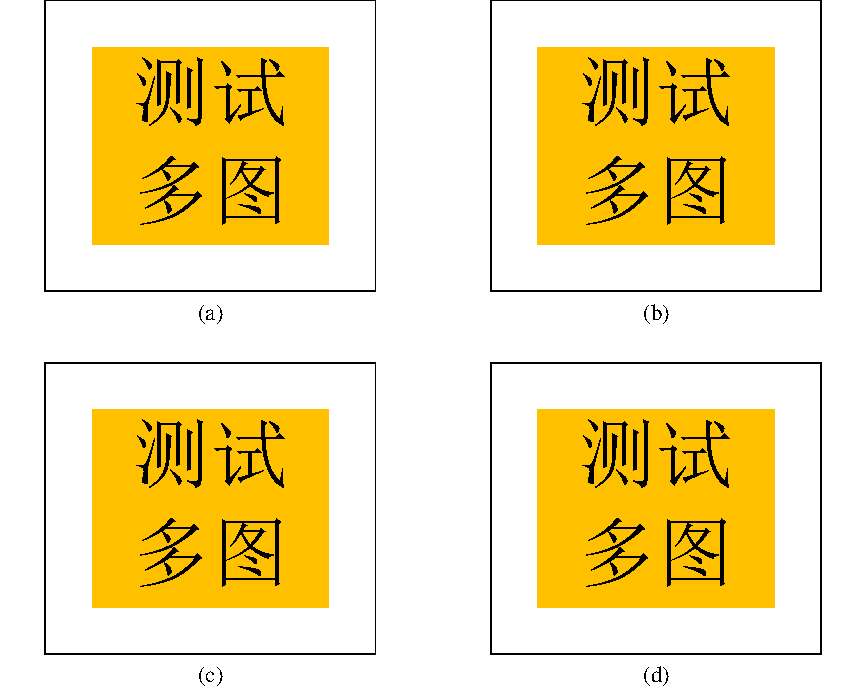
\includegraphics[width=0.85\textwidth]{figures/test-new-panels-abcd.pdf}
 \FigureCaption{多图 PDF 四联排版测试}{Four panel layout test from the new PDF}\label{fig:single}
\end{figure}
表~\ref{tab:results}的结果仅用于验证显示格式；图~\ref{fig:single}将新提供的多图 PDF 测试素材排成两行两列，并在各子图下方居中放置（a）至（d）。标号包含在组合 PDF 中，转换后与各子图保持相对位置。与第一章 PNG 图~\ref{fig:abcd}及第二章 JPG 图~\ref{fig:six}的跨章引用应指向不同图号。

进一步测试较长正文段落时，文字应沿统一版心排列，而不是通过逐行插入硬换行模拟 PDF。这样修改 TeX 内容后，Word 仍能自然重新排版。由于两种排版引擎的字距和断行规则不同，个别行末位置可能不同，但不应出现图片裁切、表格越界、编号错章或错误的超链接颜色。参考文献引用再次覆盖连续组合\cite{hu2019,astrom2008,zhou2016}和非连续组合\cite{he2016,hu2019,achenbach1973}。
\section{本章小结}
这里填写本章小结。
本章覆盖优化公式、约束公式、四列表格、独立图片与跨章交叉引用。三章共同构成可重复的转换回归样例，后续增加新内容时可先运行这些测试，检查参考文献顺序、子图标注、页码与图表编号是否保持稳定。

\chapter{长公式与多行公式测试}
本章用于检查长分数线、长根号及多行公式的边界。式~\eqref{eq:long-fraction}和式~\eqref{eq:long-system}的引用应保持可跳转。

\begin{equation}
 R=\frac{\sum_{i=1}^{N}w_i\left(x_i-\bar{x}\right)^2+\sum_{j=1}^{M}v_j\left(y_j-\bar{y}\right)^2}{\sqrt{\sum_{i=1}^{N}w_i^2+\sum_{j=1}^{M}v_j^2}+\alpha+\beta}.
 \label{eq:long-fraction}
\end{equation}

下面的分数线接近版心宽度，用于检查长横线及右侧编号是否分离。
\begin{equation}
 Q=\frac{a_1x_1+a_2x_2+a_3x_3+a_4x_4+a_5x_5+a_6x_6+a_7x_7+a_8x_8+a_9x_9+a_{10}x_{10}}{b_1y_1+b_2y_2+b_3y_3+b_4y_4+b_5y_5+b_6y_6}.
 \label{eq:wide-bar}
\end{equation}

长根号应完整覆盖被开方项，并保留上下标。
\begin{equation}
 D=\sqrt{\sum_{i=1}^{N}\left(a_i x_i+b_i y_i+c_i z_i-d_i\right)^2+\lambda\sum_{j=1}^{M}\left(p_j-q_j\right)^2}.
 \label{eq:long-root}
\end{equation}

下面的四行表达式共用一个编号，等号列应对齐。
\begin{equation}
 \begin{aligned}
 J(\mathbf{x})&=\frac{1}{2}\|A\mathbf{x}-\mathbf{b}\|_2^2+\lambda\|\mathbf{x}\|_2^2,\\
 \nabla J(\mathbf{x})&=A^{\mathsf{T}}(A\mathbf{x}-\mathbf{b})+2\lambda\mathbf{x},\\
 H(\mathbf{x})&=A^{\mathsf{T}}A+2\lambda I,\\
 \mathbf{x}_{k+1}&=\mathbf{x}_k-\eta H(\mathbf{x}_k)^{-1}\nabla J(\mathbf{x}_k).
 \end{aligned}
 \label{eq:long-system}
\end{equation}

以下六行分段形式用于检查公式高度及分页。
\begin{equation}
 f(x)=\begin{cases}
 0,&x<-2,\\
 x+2,&-2\leq x<-1,\\
 x^2,&-1\leq x<0,\\
 \exp(-x),&0\leq x<1,\\
 \frac{1}{1+x^2},&1\leq x<2,\\
 1,&x\geq2.
 \end{cases}
 \label{eq:long-cases}
\end{equation}

表格中的分式和根号使用小字号样式，不应改变三线表宽度。
\begin{table}[htbp]
 \centering
 \TableCaption{公式样式测试}{Equation style test}
 \begin{tabularx}{\textwidth}{YY}
 \toprule
 指标 & 表达式 \\
 \midrule
 方差 & $\frac{1}{N}\sum_{i=1}^{N}(x_i-\bar{x})^2$ \\
 距离 & $\sqrt{\sum_{j=1}^{M}(p_j-q_j)^2}$ \\
 \bottomrule
 \end{tabularx}
\end{table}

以上公式和正文 $\frac{a+b}{c+d}$ 同时出现时，应分别采用对应的字号，并保持引用~\eqref{eq:long-system}及~\eqref{eq:long-cases}正确。
\appendix
\chapter{补充材料}
这里填写推导、程序说明或补充图表。
附录补充误差指标的定义，并复用正文文献\cite{zhou2016}。附录编号应独立于正文第三章，不得继续显示为第三章编号。
\begin{equation}
 \mathrm{RMSE}=\sqrt{\frac{1}{n}\sum_{i=1}^{n}(y_i-\hat y_i)^2}.\label{eq:rmse}
\end{equation}

\backmatter
\printbibliography[heading=bibintoc,title={参考文献}]

\ThesisHeading{攻读博士学位期间的科研成果}
\noindent\textbf{已发表的论文：}填写论文清单。\par
\noindent\textbf{已授权的专利：}填写专利清单。\par
\noindent\textbf{已参与的项目：}填写项目清单。

\ThesisHeading{致\quad 谢}
这里填写致谢内容。

\end{document}
